\section{Theorie}
\label{sec:Theorie}

\subsection{Radioaktiver Zerfall durch Kernrekationen mit Neutronen}

Zur Herstellung instabiler und damit radioaktiver Nuklide werden Atome eines stabilen Elements mit Neutronen beschossen. 
Der Vorteil von Neutronen ist, dass sie nicht geladen sind und somit nicht die Coulomb-Barriere überwinden müssen, die 
für geladene Teilchen einen bemerkenswerten Unterschied machen würde. 
Wenn eine Reaktion stattfindet, nimmt der Kern das Neutron auf; die kinetische Energie wird fast vollständig auf alle vorhandenen Nukleonen 
verteilt. Der Kern befindet sich damit im angeregten Zustand -- für eine Zeitspanne von etwa $\SI{e-16}{\second}$. 
Dann geht er unter Emission eines $\symup{\gamma}$-Quants wieder in seinen Grundzustand über und der vorher stabile 
Atomkern hat sich in einen instabilen durch das gestiegene Verhältnis von Neutronenzahl zur Kernladungszahl umgewandelt. 
An dieser Stelle beginnt der radioaktive Zerfall, der hier untersucht werden soll. 
Ein Neutron des Nuklids wandelt sich unter Emission eines Elektrons und eines Elektron-Antineutrinos in ein Proton um, 
ein Kern einer um eins höheren Ordnungszahl entsteht. 
Die Reaktion sieht im Allgemeinen so
\begin{equation}
%    \ce{^m_zA + ^1_0 n -> ^{m+1}_zA* -> ^{m+1}_zA +\gamma -> ^{m+1}_{z+1}A + e- + \bar{\symup{\nu}}_e}
    \ce{^m_z A + ^1_0 n -> ^{m+1}_zA^* -> ^{m+1}_zA  +\symup{\gamma} -> ^{m+1}_{z+1}A +e- + \bar{\symup{\nu}}_e}
    \label{eqn:allgZerfall}
\end{equation}
aus, wobei das Sternchen $\*$ den angeregten Zustand des Kerns indiziert.
Überschüssige Energie beziehungsweise Massendifferenzen werden in Bewegungsenergie der Kerne und die Bildung von Antineutrinos $\bar{\symup{\nu}}_e$ 
gemäß der Masse-Energie-Beziehung nach Einstein $\Delta E=\Delta m c^2$ ineinander umgewandelt\cite{Versuchsanleitung}.

\subsection{Wirkungsquerschnitt}

Der Wirkungsquerschnitt $\sigma$ ist ein Maß dafür, wie wahrscheinlich ein Stoß von zwei Teilchen ist. 
Eine andere Umschreibung für den Wirkungsquerschnitt wäre, dass sie die Fläche darstellt, die ein Nukleon haben müsste, 
damit der Beschuss eines Neutrons auf die Fläche jedes Mal zu einem Einfang führt. 
Ist die Geschwindigkeit des kollidierenden Teilchens eher groß, können Interferenz- und Streueffekte vernachlässigt werden
und der Wirkungsquerschnitt kann anschaulich als die Fläche angesehen werden, die anteilmäßig von den Nukliden eingenommen wird. 
Je zahlreicher und größer die Nuklide sind, umso mehr nehmen sie prozentual an Fläche und somit an Stoßfläche ein. 
Ist hingegen die Geschwindigkeit eher gering, sorgen Streueffekte des Teilchens an den Nukliden dafür, dass die Wahrscheinlichkeit 
eines Stoßes sehr viel größer wird, als es die geometrische Betrachtung glauben machen würde\cite{Versuchsanleitung}. 

Diese Unterscheidung nach der Geschwindigkeit $v$ kann auf die Wellenlänge $\lambda$ mithilfe der De-Broglie-Beziehung
\begin{equation*}
    \lambda = \frac{\symup{h}}{m_\text{n}v}
\end{equation*}
übertragen werden, wobei $m_\text{n}$ die Masse eines Neutrons ist und das Planck'sche Wirkungsquantum durch ${\symup{h}=\SI{6.62607004e-34}{\joule\second}}$ \cite{scipy} gegeben ist. 
So kann jedem Neutron mit einer bestimmten Wellenlänge eine Geschwindigkeit zugeordnet werden. 
Zur Einordnung der Größe wird hier der Kernradius verwendet; ist die Wellenlänge sehr viel kleiner als der Kernradius ($\approx \SI{e-12}{\centi\meter}$), 
können die Streueffekte vernächlässigt werden und die geometrische Betrachtung des Wirkungsquerschnitts genügt. 

Die Absorption wird genau dann maximal -- Stichwort Resonanzabsorption --, wenn die Energie des Neutrons gerade der Energiedifferenz 
der zwei Niveaus des Atomkerns entspricht. Mithilfe einer harmonischen Annäherung und mit quantenmechanischen Annahmen begründet 
sich die sogenannte Breit-Wigner-Formel; diese sagt eine umgekehrte Proportionalität des Wirkungsquerschnitts und damit der 
Absorption der Strahlung zur Energie beziehungsweise Geschwindigkeit des Neutrons voraus
\begin{equation*}
    \sigma \propto \frac{1}{\sqrt{E}} \propto \frac{1}{v} \,,
\end{equation*}
was sich mit den vorangestellten Überlegungen deckt\cite{Versuchsanleitung}. 
Für eine hohe Reaktanz sollte die Energie der Neutronen somit eher gering gehalten werden.

\subsection{Erzeugung niederenergetischer Neutronen}

Neutronen haben eine begrenzte Lebensdauer, weshalb sie direkt vor der Messung hergestellt werden müssen. 
Die Reaktion 
\begin{equation*}
    \ce{^9_4Be + ^4_2 \symup{\alpha} -> ^{12}_6C + ^1_0n}
\end{equation*}
wird in diesem Experiment verwendet. 
Zerfallende $\ce{^{226}Ra}$-Kerne emittieren die $\alpha$-Teilchen, die auf $\ce{^9Be}$-Kerne gelenkt werden. 
Die darauffolgende Kernrekation sorgt für die Produktion von freien Neutronen und die Umwandlung der Nuklide in $\ce{^{12}C}$-Kerne. 

Da die Neutronen an dem Punkt noch eine Energie von maximal $\SI{13.7}{\mega\electronvolt}$ aufweisen, müssen sie 
entsprechend gebremst werden, um die für das Experiment günstige niedrige Geschwindigkeit zu erreichen. 
Deshalb wird die Neutronenquelle mit Paraffin ummantelt. Die darin enthaltenen leichten Wasserstoffkerne sorgen für einen 
möglichst großen Energieübertrag, wenn die Neutronen elastisch mit ihnen zusammenstoßen. 
Die Stöße finden solange statt, bis sich die Energie gleichmäßg auf die Teilchen verteilt und die Neutronen damit
die mittlere Energie der sie umgebenden Moleküle annehmen. Dies entspricht bei einer Temperatur von ${T=\SI{290}{\kelvin}}$ 
einer Energie von ${E=\SI{0.025}{\electronvolt}}$ und einer Geschwindigkeit von $v=\SI{2.2e3}{\meter\per\second}$\cite{Versuchsanleitung}. 

\subsection{Zerfall instabiler Isotope}
\label{sub:keineAhnung}

Bei der Messung werden zwei verschiedene Elemente untersucht, die jeweils einem leicht unterschiedlichen Zerfallsschema folgen. 

Allgemein lässt sich jedoch ein exponentieller Verlauf des radioaktiven Zerfalls feststellen. So wird für gewöhnlich die Anzahl der noch nicht zerfallenen Kerne $N(t)$ über 
\begin{equation*}
    N(t)=N_0 \cdot \symup{e}^{-\lambda t}
\end{equation*}
dargestellt; $\lambda$ ist die sogenannte Zerfallskonstante und der Zusammenhang zur Halbwertszeit $\tau$ lässt sich mit dem 
Ansatz $N(\tau)=\sfrac{N_0}{2}$ zu 
\begin{equation*}
    \tau=\frac{\ln 2}{\lambda}
\end{equation*}
herstellen.

Für die Messung ist $N(t)$ eine schwierig zu handhabene Größe\cite{Versuchsanleitung}, weshalb auf die Anzahl $N(\Delta t)$ in einem festen Zeitintervall $\Delta t$ zurückgegriffen wird. 
Daraus ergibt sich mit ${N_{\Delta t}(t) := N(t)-N(t+\Delta t)}$ der Zusammenhang
\begin{equation}
    \ln N_{\Delta t}(t) = \ln (N_0 (1-\symup{e}^{-\lambda \Delta t})) - \lambda t \,,
    \label{eqn:linRegr}
\end{equation}
was für eine lineare Ausgleichsrechnung in der Auswertung genutzt werden kann. 
Auf der rechten Seite ist ausschließlich die Zeit $t$ variabel, weshalb durch den Vergleich mit einer Geradengleichung $y=m\cdot x +b$ sich die Beziehungen 
\begin{align*}
    y&=\ln N_{\Delta t}(t) &\qquad \qquad x&=t \\
    m&=- \lambda & \qquad \qquad b&=\ln (N_0 (1-\symup{e}^{-\lambda \Delta t}))
\end{align*}
herstellen lassen.

Mit diesem Wissen wird zuerst das Isotop $\ce{^{51}V}$ betrachtet. Es zerfällt nach dem in \eqref{eqn:allgZerfall} gezeigten Muster\cite{Versuchsanleitung}:
\begin{equation*}
    \ce{^{51}_{23}V + ^1_0n -> ^{52}_{23}V -> ^{52}_{24}Cr + e- + \bar{\symup{\nu}}_e}
\end{equation*}
Die Halbwertszeit dieses Zerfalls lässt sich mithilfe der weiter oben beschriebenen linearen Ausgleichsrechnung bestimmen. 

Bei dem zweiten zu untersuchenden Isotop, $\ce{^{103}_{45}Rh}$ finden jedoch zwei Zerfälle statt, die bei der Messung und 
Auswertung der emittierten Strahlen berücksichtigt und unterschieden werden müssen. Die jeweiligen Halbwertszeiten weisen ebenfalls große Unterschiede auf.  
$90\%$ der Nuklide zerfällt wie bereits aus \eqref{eqn:allgZerfall} bekannt. $10\%$ zerfallen in das isomere $\ce{^{104i}Rh}$, 
welches sich in Massen- und Ordnungszahl von $\ce{^{104}Rh}$ nicht unterscheidet. 
Jedoch ist die Anordnung der Nukleonen im Kern anders, was eine starke Verringerung der Übergangswahrscheinlichkeit zwischen den 
Energieniveaus zur Folge hat. 
Dadurch verlängert sich die Zeit des Übergangs vom energetisch höheren Nuklid zum energetisch niedrigeren unter Aussendung eines 
$\gamma$-Quants auf mehrere Sekunden -- zur Erinnerung: Normalerweise geschieht dies in Zeiten von etwa $\SI{e-16}{\second}$. 
Dadurch ergeben sich die beiden Zerfallsgleichungen
\begin{equation}
    \ce{^{103}_{45}Rh + ^1_0n -> ^{104}_{45}Rh -> ^{104}_{46}Pd + e- + \bar{\symup{\nu}}_e}
\end{equation}
mit einer Wahrscheinlichkeit von $90\%$ und 
\begin{equation}
    \ce{^{103}_{45}Rh + ^1_0n -> ^{104i}_{45}Rh -> ^{104}_{45}Rh + \symup{\gamma} -> ^{104}_{46}Pd + e- + \bar{\symup{\nu}}_e}
\end{equation}
mit einer Wahrscheinlichkeit von $10\%$\cite{Versuchsanleitung}.

Aufgrund der beiden ablaufenden Prozesse wird sich in etwa der in Abbildung \ref{fig:zweiZerfaelle} dargestellte Verlauf ergeben. 
\begin{figure}
    \centering
    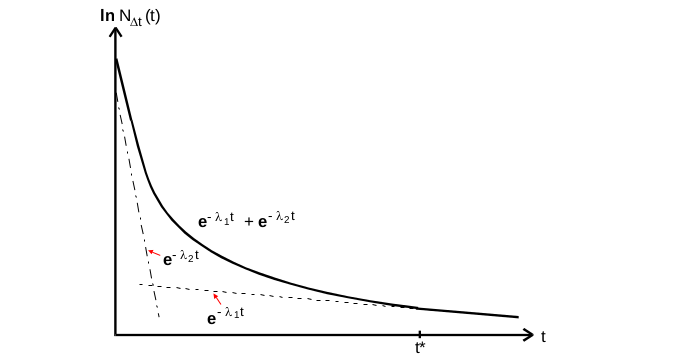
\includegraphics[width=\textwidth]{plots/zweiZerfaelle.png}
    \caption{Die Zerfallskurve zweier Isotope desselben Präparats\cite{Versuchsanleitung}.}
    \label{fig:zweiZerfaelle}
\end{figure}
Voraussetzung hierfür ist eine deutlich zu unterscheidende Halbwertszeit und Zerfallskonstante. 
Nur dann kann ab einer hinreichend großen Zeit $t^*$ ein annähernd linearer Verlauf der Kurve verifiziert werden, die 
aus dem zweiten, länger dauernden Zerfall herrührt. Für die Werte mit $t>t^*$ kann die Ausgleichsrechnung wie bei Vadium 
durchgeführt und somit die Zerfallskonstante für den zweiten Zerfall bestimmt werden. 
Danach wird von den Messwerten die ermittelte Ausgleichskurve abgezogen, damit die durch den ersten, langsameren Zerfall 
entstandenen Emissionen ausgewertet werden können. 
Hier muss beachtet werden, dass das auszuwertende Zeitintervall des ersten Zerfalls genügend Abstand zu $t^*$ hat, weil sich 
sonst durch statistische Fehler 
\begin{equation*}
    N_{\Delta t}(t)-N_{\Delta t,2}(t) <0
\end{equation*}
ergeben könnte\cite{Versuchsanleitung}.